% Options for packages loaded elsewhere
\PassOptionsToPackage{unicode}{hyperref}
\PassOptionsToPackage{hyphens}{url}
%
\documentclass[
]{article}
\usepackage{lmodern}
\usepackage{amssymb,amsmath}
\usepackage{ifxetex,ifluatex}
\ifnum 0\ifxetex 1\fi\ifluatex 1\fi=0 % if pdftex
  \usepackage[T1]{fontenc}
  \usepackage[utf8]{inputenc}
  \usepackage{textcomp} % provide euro and other symbols
\else % if luatex or xetex
  \usepackage{unicode-math}
  \defaultfontfeatures{Scale=MatchLowercase}
  \defaultfontfeatures[\rmfamily]{Ligatures=TeX,Scale=1}
\fi
% Use upquote if available, for straight quotes in verbatim environments
\IfFileExists{upquote.sty}{\usepackage{upquote}}{}
\IfFileExists{microtype.sty}{% use microtype if available
  \usepackage[]{microtype}
  \UseMicrotypeSet[protrusion]{basicmath} % disable protrusion for tt fonts
}{}
\makeatletter
\@ifundefined{KOMAClassName}{% if non-KOMA class
  \IfFileExists{parskip.sty}{%
    \usepackage{parskip}
  }{% else
    \setlength{\parindent}{0pt}
    \setlength{\parskip}{6pt plus 2pt minus 1pt}}
}{% if KOMA class
  \KOMAoptions{parskip=half}}
\makeatother
\usepackage{xcolor}
\IfFileExists{xurl.sty}{\usepackage{xurl}}{} % add URL line breaks if available
\IfFileExists{bookmark.sty}{\usepackage{bookmark}}{\usepackage{hyperref}}
\hypersetup{
  pdftitle={Final Project - OSU Building Data Analysis},
  pdfauthor={Jack Woods},
  hidelinks,
  pdfcreator={LaTeX via pandoc}}
\urlstyle{same} % disable monospaced font for URLs
\usepackage[margin=1in]{geometry}
\usepackage{graphicx,grffile}
\makeatletter
\def\maxwidth{\ifdim\Gin@nat@width>\linewidth\linewidth\else\Gin@nat@width\fi}
\def\maxheight{\ifdim\Gin@nat@height>\textheight\textheight\else\Gin@nat@height\fi}
\makeatother
% Scale images if necessary, so that they will not overflow the page
% margins by default, and it is still possible to overwrite the defaults
% using explicit options in \includegraphics[width, height, ...]{}
\setkeys{Gin}{width=\maxwidth,height=\maxheight,keepaspectratio}
% Set default figure placement to htbp
\makeatletter
\def\fps@figure{htbp}
\makeatother
\setlength{\emergencystretch}{3em} % prevent overfull lines
\providecommand{\tightlist}{%
  \setlength{\itemsep}{0pt}\setlength{\parskip}{0pt}}
\setcounter{secnumdepth}{-\maxdimen} % remove section numbering
% https://github.com/rstudio/rmarkdown/issues/337
\let\rmarkdownfootnote\footnote%
\def\footnote{\protect\rmarkdownfootnote}

% https://github.com/rstudio/rmarkdown/pull/252
\usepackage{titling}
\setlength{\droptitle}{-2em}

\pretitle{\vspace{\droptitle}\centering\huge}
\posttitle{\par}

\preauthor{\centering\large\emph}
\postauthor{\par}

\predate{\centering\large\emph}
\postdate{\par}

\title{Final Project - OSU Building Data Analysis}
\author{Jack Woods}
\date{3/13/2020}

\begin{document}
\maketitle

\hypertarget{introduction}{%
\section{Introduction}\label{introduction}}

In 2007, Oregon State University (OSU) President Ed Ray signed the
American College and University Presidents Climate Commitment, pledging
institution-wide carbon neutrality by 2025. Normalized for growth, OSU
has since reduced carbon emissions by 41\% per student per square foot
of building space; however, greenhouse gas emissions have only declined
by 12\% overall. OSU's current annual carbon footprint is equivalent to
over 15,000 average American homes, totalling over 134,000 metric tons
of \(CO_2e\) (\(CO_2\) equivalent emissions). Although significant
progress has been made, carbon neutrality will not be achieved by 2025
unless additional emissions reductions can be achieved.

\begin{figure}
\centering
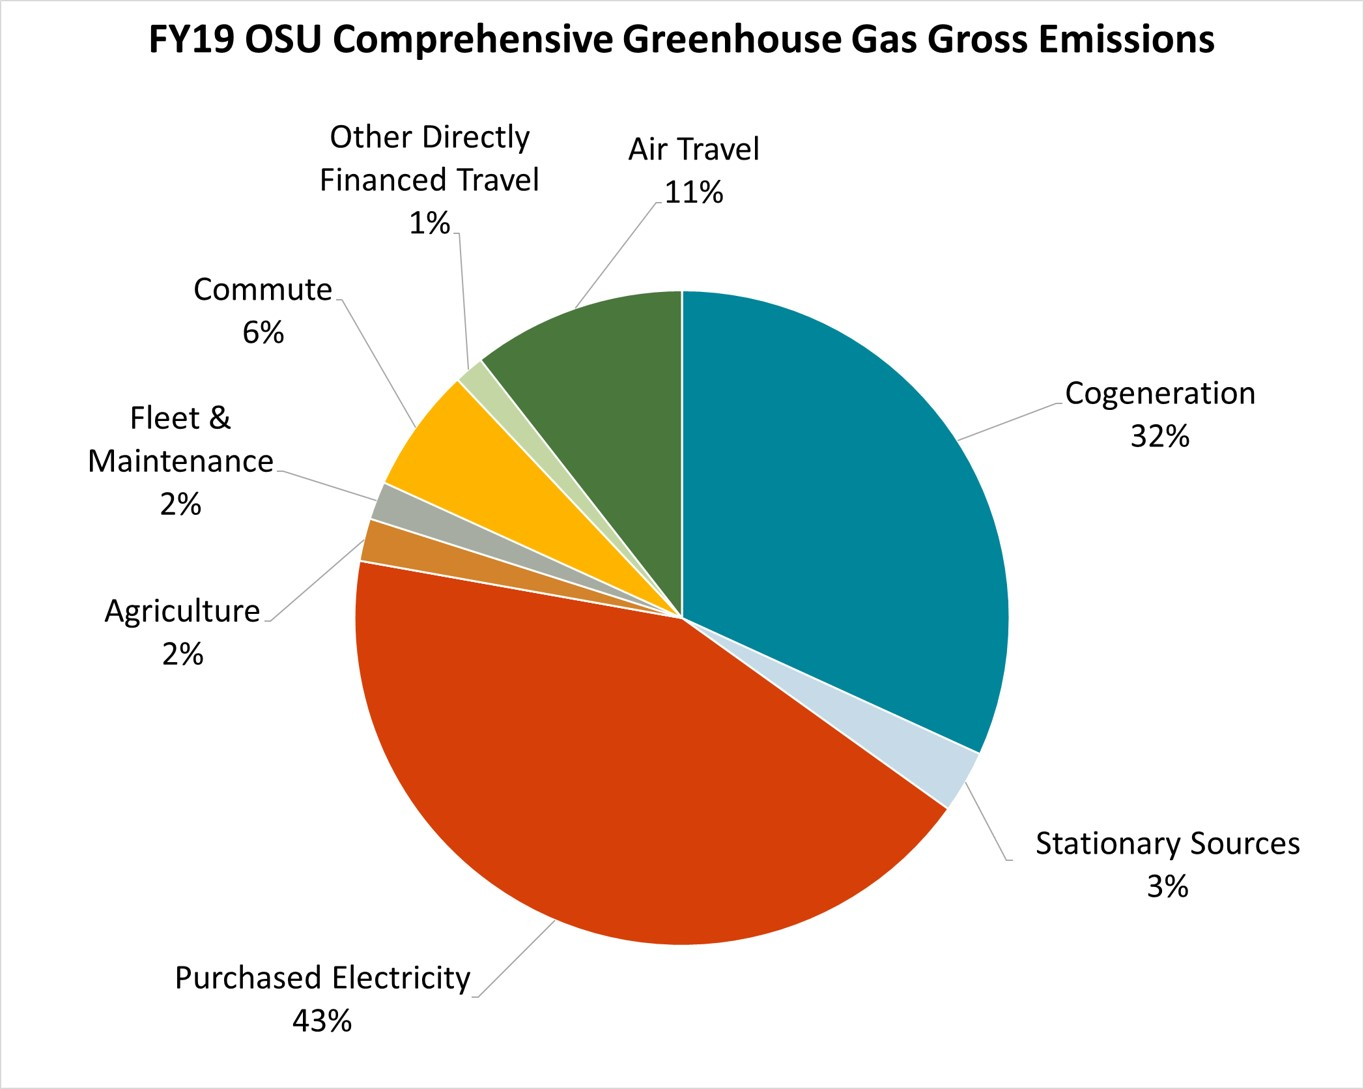
\includegraphics{../documents/pie_gross_emissions.jpg}
\caption{Emissions Pie Chart}
\end{figure}

\begin{figure}
\centering
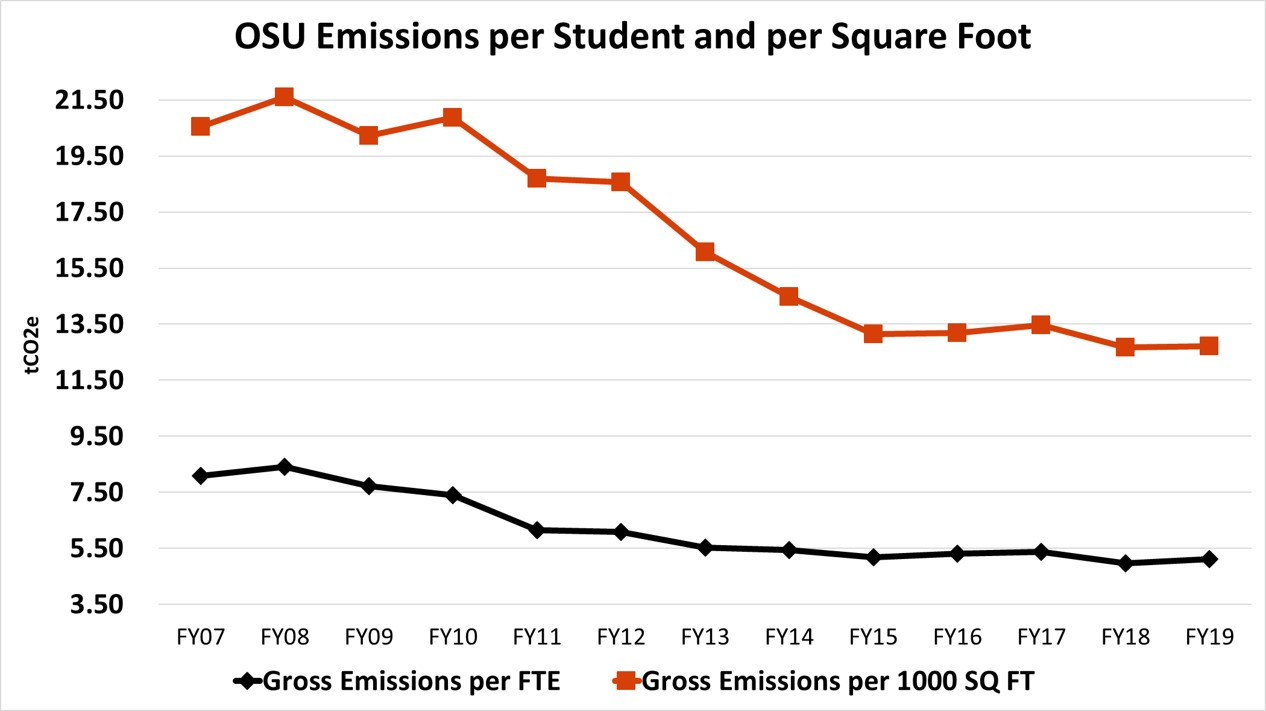
\includegraphics{../documents/normalized1.jpg}
\caption{Emissions Per Student}
\end{figure}

The OSU Sustainability Office reports that electricity consumption
accounts for approximately 75\% of OSU's carbon emissions. Thus,
understanding electricity consumption patterns is a critical step
towards advancing OSU's emissions reduction initiatives. As Climate
Change contributes to increasingly unstable climate/weather/temperatures
worldwide, understanding the connection between OSU's electricity
consumption and Corvallis's weather is critical for determining:

\begin{itemize}
\tightlist
\item
  The effects of Climate Change on OSU's electricity consumption
  patterns.
\item
  Whether Global Warming/Climate Change will cause campus-wide energy
  consumption to decrease or increase.
\item
  Other patterns in daily, weekly, monthly, quarterly, or seasonal
  consumption.
\end{itemize}

This project aims to connect weather conditions to energy consumption in
buildings across OSU's Corvallis Campus by comparing energy, building,
and weather data from June 1, 2018 to March 7, 2020. Daily electricity
consumption data is limited by the availability of real time electricity
meter reporting hardware. Only approximately 30 buildings on OSU's
campus have data acquisition servers installed, which severely limits
the amount of data available. Of these 30 buildings, a subset were
selected to ensure that academic, residential, sports-related, and
events spaces were represented in our sample.

\hypertarget{methods}{%
\section{Methods}\label{methods}}

\hypertarget{data-collection}{%
\subsection{Data Collection}\label{data-collection}}

Weather data was requested through the U.S. National Oceanic and
Atmospheric Administration's (NOAA) National Centers for Environmental
Information Climate Data Online Search platform. Automated precipitation
and temperature data were collected by an automated weather station
(NOAA ID: USW00004236) located near Corvallis, OR. Electricity
consumption data was collected using Acquisuite Data Acquisition Servers
connected to electrical meters in OSU buildings via a modbus connection.
The data was aggregated in a cloud database using OSU's Energy Dashboard
web application. Building square footage data was provided by request by
the OSU Sustainability Office.

\hypertarget{design}{%
\subsection{Design}\label{design}}

In \textbf{Figure 1}, many trends can be observed:

\begin{itemize}
\tightlist
\item
  As \emph{TMIN} and \emph{TMAX} increase, \emph{epsf} decreases.
\item
  Different buildings exhibit different energy consumption densities per
  square foot, indicating that \emph{Building} may play a large role in
  determining \emph{epsf}. This is likely due to the fact that buildings
  were constructed over a long time period and contain unique HVAC
  systems of varying efficiency and complexity.
\item
  Electricity consumption trends vary between buildings. Some buildings
  exhibit an increase in electricity consumption above 70 degrees
  Fahrenheit, resulting in a concave upward curvature in the
  scatterplot. Others do not exhibit the same increase. This is likely a
  result of air conditioning systems that are installed on some, but not
  all, buildings.
\end{itemize}

\textbf{Figure 2} and \textbf{Figure 3} reveal that electricity
consumption trends vary widely month-to-month and day-to-day. This
reflects building occupancy trends across campus. During summer months
and December, typical building utilization is disrupted by students
leaving for breaks. This is most likely what is reflected in building
electricity consumption.

\textbf{Figure 5} depicts Buxton Hall and the International Living
Learning Center's (ILLC) electricity consumption. Note the significant
decline in electricity consumption during Summer and Winter Break (June,
July, August, September, and December). Although the International
Living Learning Center(ILLC) is classified as a residence hall in our
dataset, the ILLC contains a coffee shop, convenience store, multiple
classrooms, and many offices on the first floor. In contrast, Buxton
Hall is strictly a residence hall. I believe the difference in energy
consumption trends is explained by the usage trends of the various
spaces within the building. This information is captured on a macro
scale by the \emph{Type} effect, but is not captured on a micro scale.

\textbf{Figure 5} plots \emph{epsf} and daily \emph{PRCP} in Corvallis
and reveals no clear correlation between precipitation and electricity
consumption. \textbf{Figure 6} illustrates little to no interaction
between \emph{Temperature} and \emph{PRCP}. Although I initially thought
that the quantity of precipitation would be correlated with higher
electricity consumption (since students would likely spend more time
indoors), this does not appear to be true.

To summarize everything:

\begin{itemize}
\tightlist
\item
  There is a correlation between temperature and electricity
  consumption.
\item
  Each building and building type have unique consumption trends.
\item
  Buildings exhibit different energy trends throughout the year.
  \emph{Month} is likely to be significant in the linear model.
\item
  Electricity consumption trends follow cyclic secondary trends on a
  weekly basis.
\end{itemize}

For this report, a least squares linear regression model will be created
to find a relationship between outside air temperature and building
electricity consumption. In this case, a linear model is a convenient
tool because it provides mechanisms which allow an analyst to study the
effect of one explanatory variable on the response variable while
holding all other factors constant. For example, a slope coefficient
would provide a sufficient link between changes in electricity
consumption explained by changes in outside air temperature.

\hypertarget{the-model}{%
\subsection{The Model}\label{the-model}}

The initial ANOVA test found \emph{PRCP}, \emph{Type}, and the squared
\emph{TMAX} terms to be insignificant. Interestingly, the other
temperatures appear to be significant. This is likely because the
minimum and maximum temperatures are highly correlated with one another
(Correlation is 0.765271. Removing \emph{PRCP} and \emph{Type} from the
model, we obtain:

The ESS F-test results provide overwhelming evidence in favor of the
reduced model. This reveals that categorizing the buildings by ``Type''
(Academic, Residential, etc) is not useful for our analysis. This is
likely because most buildings are vastly different from one another,
even within the same category. Additionally, the categories do not
accurately account for the various spaces within each building (such as
the cafe in LINC or the offices in some of the residence halls).

This model does not consider the correlation between temperatures,
however. To construct the final model, we remove the squared \emph{TMAX}
term and create an interaction term between \emph{Building} and the
squared \emph{TMIN} term. Lastly, we introduce a interaction terms
between \emph{Building} and \emph{Month} \& \emph{dayOfWeek}.

The interaction terms were included in this model because:

\begin{itemize}
\tightlist
\item
  Some buildings exhibited curvature in \textbf{Figure 1}, while others
  did not.
\item
  Electricity consumption in residence halls decreases significantly
  over the summer months, while academic buildings exhibit different
  effects.
\item
  Some buildings, such as residence halls, have similar occupancy on
  weekends vs weekdays while academic buildings do not.
\end{itemize}

Overall, this change improved the \(R^2\) and \(R^2_{adj}\) values
significantly.

\hypertarget{results}{%
\section{Results}\label{results}}

Overall, the final model captures electricity consumption trends
reasonably well. \textbf{Figure 7} depicts relatively consistent and
small residuals, and \textbf{Figure 8} shows predicted kWh daily
consumption for the Memorial Union. Considering that many factors (such
as building occupancy, age, and HVAC system types) were not specifically
addressed in the model, I believe the model performs well.

\hypertarget{discussion}{%
\section{Discussion}\label{discussion}}

It is important to note that inferences derived from the model will be
limited by the following:

\hypertarget{location-constraints}{%
\subsubsection{Location Constraints}\label{location-constraints}}

The data collected for this project originates at only the Corvallis
Campus. The results of this report may not accurately project
electricity consumption trends across all OSU-owned properties.
Additionally, a small subset of OSU buildings in Corvallis were used to
construct this model.

\hypertarget{limited-time-series-data}{%
\subsubsection{Limited Time-Series
Data}\label{limited-time-series-data}}

All of the data used in this report spans less than two years of
consumption data. To really understand long term electricity consumption
trends, a broader time span is required for accurate prediction.

\hypertarget{correlation-colinearity}{%
\subsubsection{Correlation \&
Colinearity}\label{correlation-colinearity}}

For simplicity, the model does not account for correlation between
neighboring time-series observations. Additionally, the model does not
consider the correlation that may exist between \emph{Temperature} \&
\emph{Month} or \emph{Temperature} and \emph{Year}.

For the purposes of this Final Project, the findings in this report are
sufficient for finding a link between climate changes and electricity
consumption trends. I do not believe the findings of this report are
sufficient grounds for institutional decision-making; however, with more
data, time, and resources, I believe a more accurate model could be
produced that accurately projects energy consumption over a longer time
interval. As OSU continues to expand smart metering programs and
develops novel ways to collect more building data (such as building
occupancy, or device-specific electric metering), an accurate model
could be created.

\hypertarget{conclusions}{%
\section{Conclusions}\label{conclusions}}

Maximum and minimum daily temperatures have a statistically significant
effect on building electricity consumption. For each 1 degree increase
in maximum temperature, facility operators can expect a 0.00004756
increase in \emph{kWh/sq. ft.} consumption campus wide. The effect of
minimum temperature changes is hard to quantify because it is almost
negligible campus wide but varies immensely by building. \textbf{Figure
9} depicts the effect of a 2 degree celsius increase in daily
temperature.

With a 2 degree Celsius increase in average temperature, OSU's facility
operators can expect an increase in electricity consumption if the mean
outside air temperature is greater than 55 F, and a decrease in
electricity consumption otherwise.

\hypertarget{informal-sources-cited}{%
\section{Informal Sources Cited}\label{informal-sources-cited}}

OSU Carbon Commitment and Emissions Statistics -
\url{https://fa.oregonstate.edu/sustainability/planning-policy-assessment/institutional-carbon-neutrality}

Carbon Emissions Breakdown -
\url{https://fa.oregonstate.edu/sustainability/planning-policy-assessment/institutional-carbon-neutrality/emissions-measurement-and}

Electricity Data -
\url{https://dashboard.sustainability.oregonstate.edu/}

Weather Data - \url{https://www.ncdc.noaa.gov/cdo-web/}

Building Square Footage and Other Data - Available upon request from the
OSU Sustainability Office. Contact Lety:
\href{mailto:leticia.cavazos@oregonstate.edu}{\nolinkurl{leticia.cavazos@oregonstate.edu}}

\end{document}
